%!TEX root = ../main.tex

\section{Введение}

\begin{frame}{Физическое явление}
\begin{block}{Электрический пробой}
	Явление резкого возрастания тока в диэлектрике при приложении электрического напряжения выше критического.
\end{block}
\begin{itemize}
	\item Рассматриваем твердый диэлектрик
	\item Деградация диэлектрических свойств материала
	\item Процесс развивается в ограниченной зоне -- канале пробоя
	\item Сложная физическая природа
\end{itemize}
\end{frame}


\begin{frame}{Математическая модель}
\begin{block}{Модель типа диффузной границы}
	Вещество находится в разных фазах. Состояние вещества описывается гладкой функцией $\phi(\vx, t)$ -- фазовым полем.
\end{block}
\begin{itemize}
	\item $\phi = 1$ -- неповрежденная среда
	\item $\phi = 0$ -- полностью разрушенная среда
	\item Зона $\phi \in (0, 1)$ -- диффузная граница
	\item На разрушение среды тратится энергия
\end{itemize}
\begin{figure}
	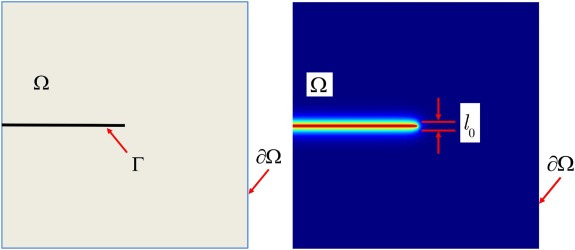
\includegraphics[width=0.5\textwidth]{figures/diffuse_edge.jpg}
\end{figure}
\end{frame}